\documentclass{article}

\usepackage[top=2.54cm, left=2.54cm, right=2.54cm, bottom=2.54cm]{geometry}
\usepackage{amsmath}
\usepackage{booktabs}
\usepackage{hyperref}
\usepackage{multicol}
\hypersetup{colorlinks=true, urlcolor=blue,}
\usepackage[svgnames]{xcolor}
\usepackage{graphicx}
\usepackage{cancel}
\usepackage{float}

\begin{document}
Jake Mathews \hfill July 3rd, 2018 \\
\hrule
\begin{center}
\large {Homework Assignment 6}\\ \large{Projectile Motion}
\end{center}
\hrule
\vspace{1pt}
\hrule height 1pt

\section{Introduction}
The goal of this assignment is to plot various 2D kinematic trajectories along its flight path in the x and y planes given an initial velocity and an angle of launch in degrees. Before that can be done though, the equation for calculating position over time must be derived from the definition of acceleration. The definition of acceleration can be given as

\begin{equation}
\label{eq:1}
a = \frac{dv}{dt}
\end{equation}
where a is acceleration and it is equal to the derivative of velocity with respect to time. From there both sides can be multiplied by $dt$ producing the following

\begin{equation}
\label{eq:2}
a \cdot dt = dv
\end{equation}

By taking the definite integral of each side, the equation is bounded to our the use case

\begin{equation}
\label{eq:3}
\int_{v_o} ^ {v} dv = \int_{t_o} ^ {t} a dt
\end{equation}
Then evaluated at its bounds, the equation becomes

\begin{equation}
\label{eq:4}
v \Big|_{v_o}^{v} = a \cdot t \Big|_{t_o}^{t}
\end{equation}
Evaluated at its bounds, the problem is clear that the change in velocity is dependent on the acceleration with respect to the change in time.

\begin{equation}
\label{eq:5}
v - v_o = a (t - t_o)
\end{equation}
However, the initial time will be 0, so that can be removed

\begin{equation}
\label{eq:6}
v - v_o = a (t - \cancel{t_o}^{0}) \rightarrow v - v_o = a \cdot t
\end{equation}
Adding initial velocity to both side produces the derivation of acceleration which is velocity

\begin{equation}
\label{eq:7}
\boxed{v = v_o + a \cdot t}
\end{equation}
The goal is still to get an equation to calculate position and not just velocity. Velocity can also be defined as

\begin{equation}
\label{eq:8}
v = \dfrac{dx}{dt}
\end{equation}
Which equates velocity to the change in position with respect to time. Substituting the final velocity in the derived equation with equation \ref{eq:8} can be seen as

\begin{equation}
\label{eq:9}
\dfrac{dx}{dt} =  v_o + a \cdot t
\end{equation}
Multiplying both sides by $dt$ to isolate $dx$ yields

\begin{equation}
\label{eq:10}
\cancel{dt} \cdot \dfrac{dx}{\cancel{dt}} =  (v_o + a \cdot t) dt \rightarrow dx =  (v_o + a \cdot t) dt
\end{equation}\\
\noindent
Then the definite integral with respect to distance and time are taken

\begin{equation}
\label{eq:11}
\int_{x_o}^{x} dx = \int_{0}^{t} (v_o + a \cdot t) dt
\end{equation}
Evaluated at its bounds reveals the derivation of position from velocity

\begin{equation}
\label{eq:12}
x\Big|_{x_o}^{x} = v_o t + \dfrac{1}{2}at^2 \rightarrow \boxed{x = x_o + v_o  t + \dfrac{1}{2}at^2}
\end{equation}
Now equations for the positions in the x-y plane must be derived separately and account for the initial angle of the trajectory

\begin{equation}
\label{eq:13}
x = x_o +  v_o  cos(\theta) t + \dfrac{1}{2}at^2
\end{equation}

\begin{equation}
\label{eq:14}
y = y_o + v_o  sin(\theta) t + \dfrac{1}{2}at^2
\end{equation}

If the initial position in in both the x and y planes are set to zero and if air resistance is ignored so there is no acceleration in the x axis in null, the equations can be simplified to

\begin{equation}
\label{eq:15}
x = \cancel{x_o} +  v_o  cos(\theta) t + \cancel{\dfrac{1}{2}at^2} \rightarrow
\boxed{x = v_o  cos(\theta) t}
\end{equation}

\begin{equation}
\label{eq:16}
y = \cancel{y_o} + v_o  sin(\theta) t + \dfrac{1}{2}at^2 \rightarrow
\boxed{y = v_o  sin(\theta) t + \dfrac{1}{2}at^2}
\end{equation}
Acceleration in the y axis remains because the projectile is subject to gravity, which assuming the projectile is on earth is $9.81 m/s^2$. These equations are what will be used in the simulation.

\pagebreak
\section{Simulation Results}
Figure \ref{fig:1} is a plot of a projectiles height from the launch site ($y$) versus its horizontal distance from the launch site ($x$)

\begin{figure}[H]
\begin{center}
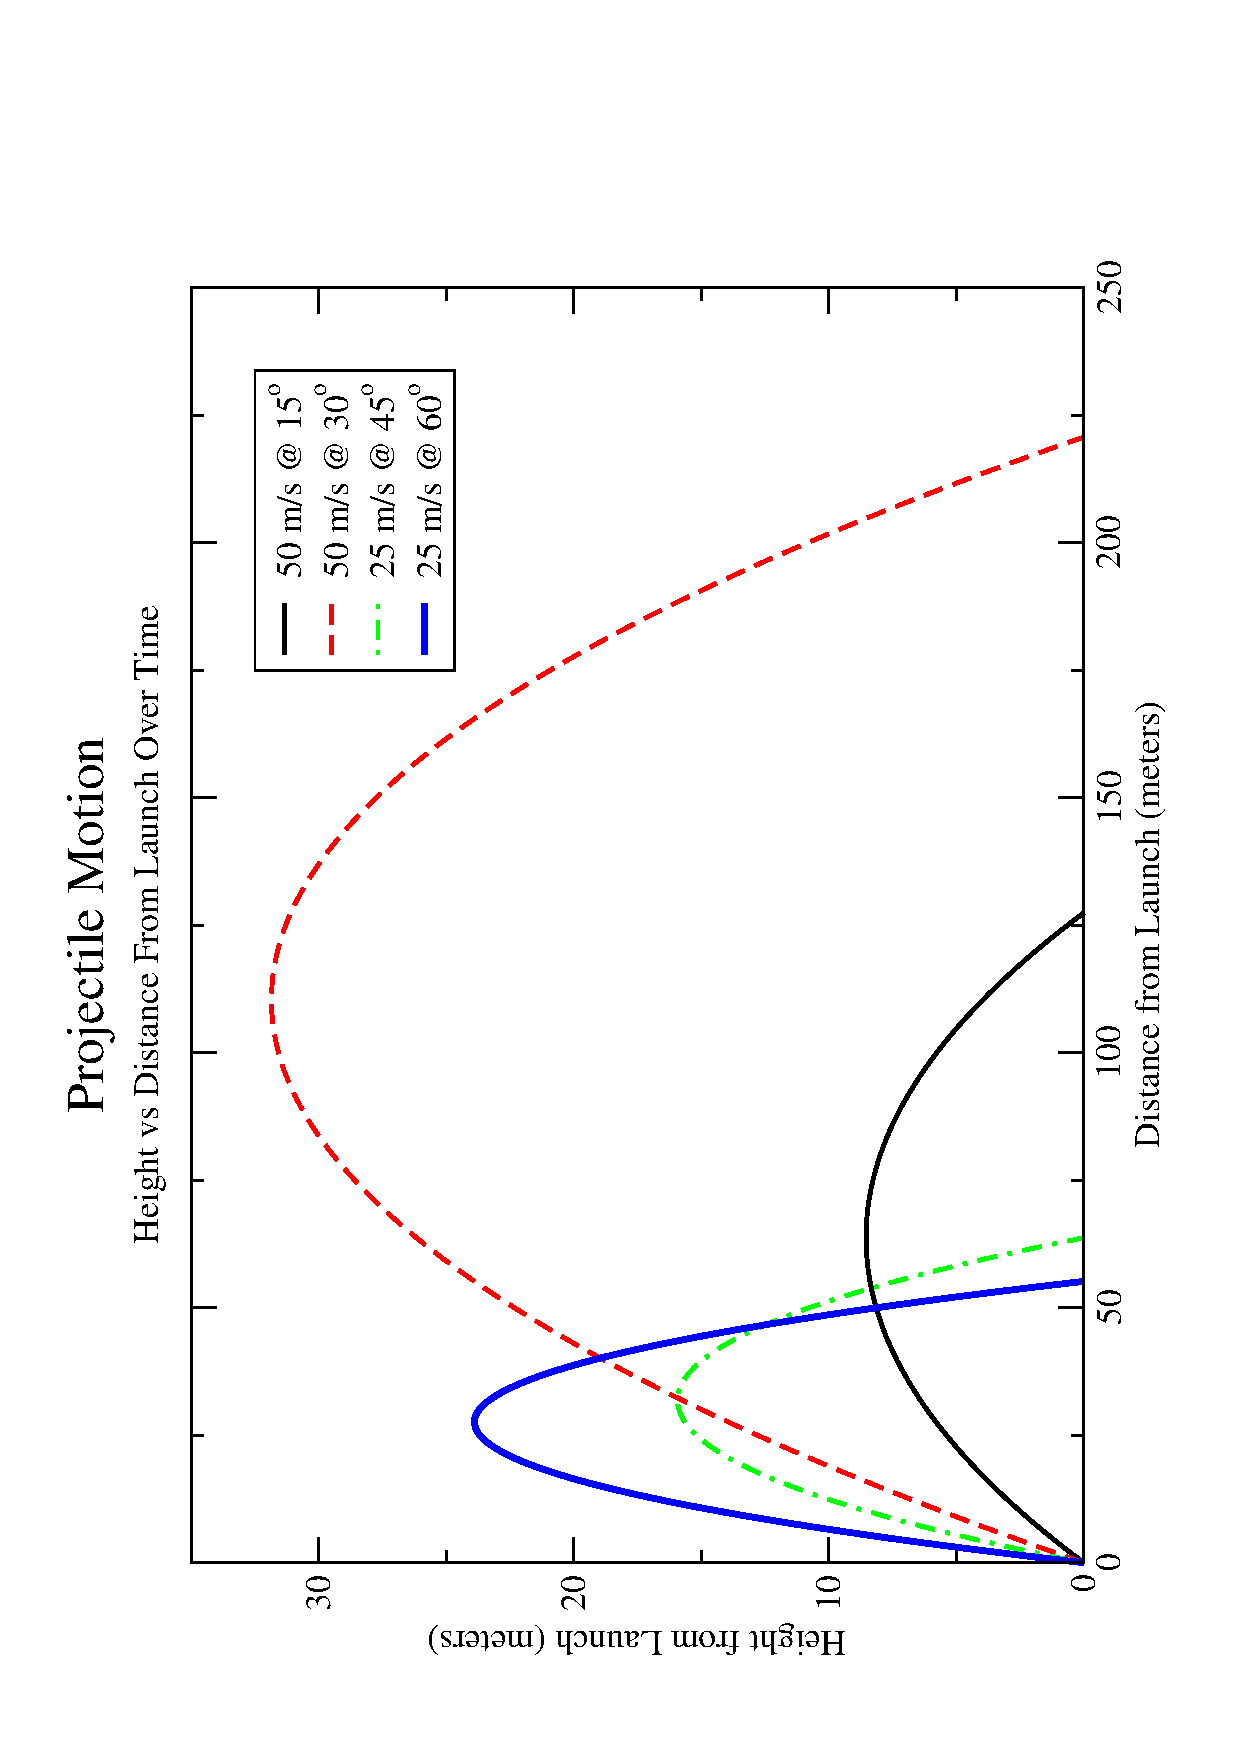
\includegraphics[scale=0.65]{./motion}
\end{center}
\caption{Projectile Motion Plot}
\label{fig:1}
\end{figure} 
\noindent 
Figure \ref{fig:1} shows the paths of four projectiles in the x-y plane. One thing this illustrates is what matters more than angle in getting distance, is the initial speed. A launched at $45^o$ should go the farthest, but a launch at only $15^o$ travels twice the distance, because it has double the speed of the projectile thrown at $45^o$ 

\begin{table}[H]
\centering
\begin{tabular}{ l l l l } 
\multicolumn{4}{c}{Table 1: Projectile Statistics}\\
\hline \hline
$Velocity$ & $Angle$ & $Max Height$ & $Time To Max Height$\\
 \hline
 $50 m/s$ & 		$15^o$ 		& 		$8.50m$ 	& 		$1.32s$\\\noalign{\smallskip}
 $50 m/s$ & 		$30^o$ 	& 		$31.86m$	& 		$2.55s$\\\noalign{\smallskip}
 $25 m/s$ & 		$45^o$ 	& 		$15.93m$ & 		$1.80s$\\\noalign{\smallskip}
 $25 m/s$ & 		$60^o$ 	& 		$23.89m$ & 	$2.21s$\\\noalign{\smallskip}
 \hline
\end{tabular}
\caption{Showing the projectile's max height and the time to max height}
\label{table:1}
\end{table}
\noindent
Although Figure \ref{fig:1} shows that although speed is far more important in distance than the angle, Table \ref{table:1} illustrates the importance of angle on air time. If the goal is to maximize the amount of time a projectile spends in the air, then the angle of the launch should also be maximized.

\section{The Code}
These simulation results are the product of a FORTRAN 90 program. The flow of the program starts off by requesting that the user enter in real numbers for the angle and initial velocity of the projectile separated by a comma. Then the program checks to see if the user input falls into one of the four predefined trajectories. The predefined trajectories can be found in Table \ref{table:1}. 

If the user has not entered in one of those trajectories, the user will be notified in the console that because what they entered is not one of those four trajectories, it will not be writing the data to a file. It will however still run the simulation and print out statics similar to the results in Table \ref{table:1}.

If the user did enter in one of the predefined trajectories, the program will record each x and y position to a data file named 'traj{angle}.dat' where {angle} is replaced with the angle of the trajectory. The .dat files can be used to run statistical analysis on and/or plot the results to a graph as seen in Figure \ref{fig:1}. The program will then print out statics similar to the results in Table \ref{table:1}.

This simulation is done be running equations \ref{eq:15} and \ref{eq:16} in a loop. In these equations, the angle and initial velocity are provided by the user. Acceleration in the case of Equation \ref{eq:16} is the gravitational constant for earth where $g = 9.81m/s^2$. The value of time is determined by the loop where the loop increments the time by $0.1s$. Each loop these values are plugged into the equations, where they may be plotted. The every loop, the y position is compared to the previous highest point, and if it is higher, the new highest point becomes the current y position and the time to reach max height becomes the current time. The loop will continue to iterate until the y position is at or below the initial start height of zero.

\end{document}
